\documentclass[11pt, oneside]{article}   	% use "amsart" instead of "article" for AMSLaTeX format
\usepackage{geometry}                		% See geometry.pdf to learn the layout options. There are lots.
\geometry{letterpaper}                   		% ... or a4paper or a5paper or ... 
%\geometry{landscape}                		% Activate for for rotated page geometry
%\usepackage[parfill]{parskip}    		% Activate to begin paragraphs with an empty line rather than an indent
\usepackage{graphicx}				% Use pdf, png, jpg, or eps§ with pdflatex; use eps in DVI mode
								% TeX will automatically convert eps --> pdf in pdflatex		
\usepackage{amssymb}
\usepackage{amsmath}
\usepackage{parskip}
\usepackage{color}
\usepackage{hyperref}

\title{Maxwell's equations}
%\author{The Author}
%\section{}
%\subsection*{}
\date{}							% Activate to display a given date or no date

\graphicspath{{/Users/telliott_admin/Tex/png/}}
% \begin{center} 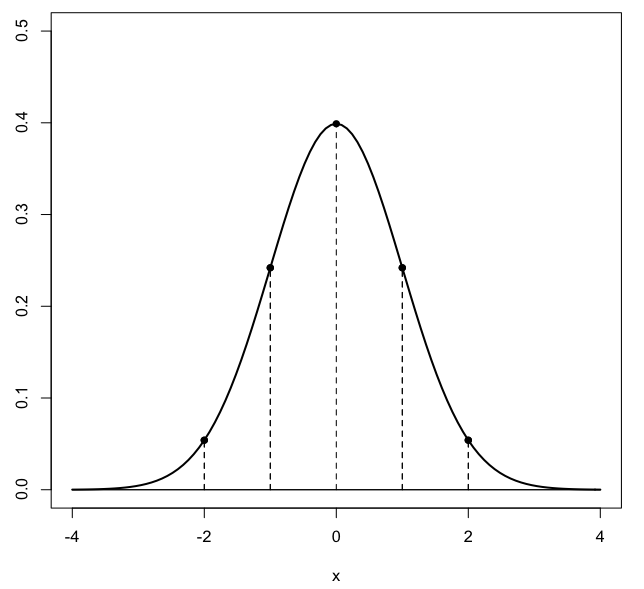
\includegraphics [scale=0.4] {gauss3.png} \end{center}
\begin{document}
\maketitle
\Large

This short write-up is a brief introduction to Maxwell's Equations.  I want to show both the "differential" and "integral" forms, and to do that we need to start with a review of the Divergence Theorem and Stokes' Theorem.  It's easiest to understand those by looking first at the 2D case using Green's Theorem.
\subsection*{Green and Stokes}
Green's Theorem applies to curves and fields that "live in the plane."  It comes in two versions.  The first one says that the work done going around a closed curve $C$ embedded in a vector field $\mathbf{F}$ is equal to the "curl" of the same field over the region enclosed by the curve.  (The curl is only defined in 3D, but here its single component is in the $z$-direction since the vector field has no $z$-component).
\[ \oint \mathbf{F} \cdot d \mathbf{r} = \iint_R \nabla \times \mathbf{F} \ dA \]
The physical meaning of this is pretty easy to understand.  If the field has some circulation (non-zero curl), then the work done will be non-zero as well.  With no circulation, there can be no (net) work.

In terms of computation, if $\mathbf{F} = \ \langle M, N \rangle$, then the left-hand side is 
\[ \oint \mathbf{F} \cdot d \mathbf{r} = \int \langle M, N \rangle \cdot \langle dx, dy \rangle \]
To actually evaluate this integral, we will need to parametrize the curve and express both $x$ and $y$ in terms of a single variable like $x$, or perhaps, $t$.

For this simple example in the plane, the curl of $\mathbf{F}$ has its only component in the $z$-direction, and its magnitude is $N_x - M_y$, so the double integral over the region is
\[ \iint_R \nabla \times \mathbf{F} \ dA = \iint (N_x - M_y) \ dx \ dy \]
This is a real double integral.

For a conservative force, the force is the gradient of some scalar function called the potential ($\mathbf{F} = \nabla \phi = \ \langle \phi_x, \phi_y \rangle$), so the curl ($\nabla \times \mathbf{F} = N_x - M_y = \phi_{yx} - \phi_{xy}$) is zero, since the mixed second derivatives of a function $\phi(x,y)$ must be equal.

In three dimensions, this becomes Stokes' Theorem:
\[ \oint_C \mathbf{F} \cdot d \mathbf{r} = \iint_S ( \nabla \times \mathbf{F}) \cdot \hat{\mathbf{n}} \ dS \]
Stokes theorem applies to a curve in space, which does not have to lie in a plane.  The theorem says that the work going around the curve is equal to the integral of the component of the curl of $\mathbf{F}$ normal to the surface, over \emph{any surface} with that curve as its boundary. 

\subsection*{Green and Divergence}
Green's Theorem for flux in the plane is
\[ \oint_C \mathbf{F} \cdot \mathbf{n} \ ds = \iint_R \nabla \cdot \mathbf{F} \ dA \]
Here, we imagine that $\mathbf{F}$ could be a velocity field of some kind, like that describing the flow of a fluid.  What the theorem says is that if there is net flow across the boundary, there has to be a source or a sink inside, depending on the sign of the flow.

As before, the left-hand integral needs to be cast in terms of a single variable through parametrization of the curve.  The right-hand side is (for $\mathbf{F} = \ \langle M, N \rangle$)
\[ \iint_R \nabla \cdot \mathbf{F} \ dA = \iint (M_x + N_y) \ dx \ dy   \]

In three dimensions, the divergence theorem is
\[ \iint_S \mathbf{F} \cdot \mathbf{n} \ dS = \iiint_V \nabla \cdot \mathbf{F} \ dV = \iiint_V (P_x + Q_y + R_z) \ dx \ dy \ dz \]
(for $\mathbf{F} = \ \langle P,Q,R \rangle$).

\subsection*{Gauss's Law}
The first of Maxwell's Equations is Gauss's Law, which says that for any surface enclosing a set of charges, the total flux of the electric field through the surface is related to the total charge inside
\[ \Phi_E = \frac{Q}{\epsilon_0} = \iint_S \mathbf{E} \cdot d\mathbf{A} \]
So, if we knew the field (magnitude and direction) at every point on the surface, then we could calculate the charge.  However, the usual situation is that we know the charge, and for a limited number of special cases we argue from symmetry that the field is everywhere perpendicular to the surface.  For example, consider a charged sphere and a Gaussian surface surrounding that sphere at a radius of $R$ from the center of the sphere.  By symmetry, the field is radial.  We write
\[ \frac{Q}{\epsilon_0} = \iint_S \mathbf{E} \cdot d\mathbf{A} \]
\[ = \iint_S E \ dA \]
We can do the last step because of the radial field.  Then
\[ = E \iint_S \ dA = E \ 4 \pi R^2 \]
Therefore,
\[ E = \frac{1}{4 \pi \epsilon_0} \ \frac{Q}{R^2} \]
which is easily transformed to Coulomb's Law when we multiply by the value of a test charge.

All of Maxwell's equations have both an integral form like
\[ \frac{Q}{\epsilon_0} = \iint_S \mathbf{E} \cdot d\mathbf{A} \]
as well as a differential form, which in this case is
\[ \nabla \cdot \mathbf{E} = \frac{\rho}{\epsilon_0} \]
The integral form integrates over some volume, the differential form refers to a small region of space and describes what the field is doing there.

The way to show the equivalence of these two forms is to go back to the divergence theorem (substituting $\mathbf{E}$ for $\mathbf{F}$)
\[ \iint_S \mathbf{E} \cdot \mathbf{n} \ dS = \iiint_V \nabla \cdot \mathbf{E} \ dV \]
Since $\mathbf{n} \ dS$ is really the same as $d\mathbf{A}$, the left-hand side is just $Q/\epsilon_0$ by the first version of the law, which means that
\[ \frac{Q}{\epsilon_0} = \iiint_V \nabla \cdot \mathbf{E} \ dV \]
And then the trick is to say that the charge is the integral of the charge density $\rho$ over the volume
\[ \frac{1}{\epsilon_0} \iiint_V \rho \ dV  = \iiint_V \nabla \cdot \mathbf{E} \ dV \]
Since the integrals are equal, so are the integrands!
\[ \frac{1}{\epsilon_0} \rho  = \nabla \cdot \mathbf{E} \]

\subsection*{Gauss's Law for magnetism}
Since there is no such thing as a "magnetic charge" or magnetic monopole
\[ \iint_S \mathbf{B} \cdot d\mathbf{A} = 0 \]
\[ \nabla \cdot \mathbf{B} = 0 \]

\subsection*{Ampere's Law}
Ampere discovered that there is a magnetic field surrounding a wire in which a current is moving
\begin{center} 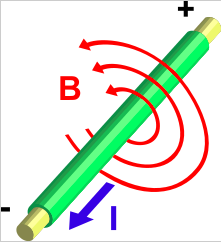
\includegraphics [scale=0.6] {ampere1.png} \end{center}
The law says that the circulation of the magnetic field surrounding a current is
\[ \oint \mathbf{B} \cdot d\mathbf{r} = \mu_0 \sum_i I_i =  \mu_0 I \]

Go back to Stokes' Theorem, and this becomes
\[  \mu_0 I = \iint_S ( \nabla \times \mathbf{B}) \cdot \hat{\mathbf{n}} \ dS \]
Recall the trick we used before.  We can view the current as the integral over the whole surface of a current density $\mathbf{j}$, so we obtain
\[  \iint_S \mu_0 \ \mathbf{j}  \cdot \hat{\mathbf{n}} \ dS = \iint_S ( \nabla \times \mathbf{B}) \cdot \hat{\mathbf{n}} \ dS \]
but if the integrals are equal, then so are the integrands.  Thus
\[  \mu_0 \ \mathbf{j}   = \nabla \times \mathbf{B} \]
Now, we're not supposed to know this yet, but later on we will find out that
\[ \frac{1}{c^2}= \epsilon_0 \ \mu_0 \]
So we can rewrite the previous result as

\[ \nabla \times \mathbf{B} = \frac{1}{c^2 \ \epsilon_0} \ \mathbf{j}  \]
or
\[ c^2 \ \nabla \times \mathbf{B} = \frac{\mathbf{j} }{\epsilon_0} \]
This equation acquires another term due to Maxwell and the "displacement current"
\[ c^2 \  \nabla \times \mathbf{B} = \frac{\mathbf{j} }{\epsilon_0} + \frac{\partial \mathbf{E}}{\partial t}  \]

\subsection*{Displacement current}
Consider a circuit containing a battery, a switch and a capacitor.  Throw the switch and the capacitor will charge.  Current flows in the circuit except across the capacitor.  According to Ampere's Law, at any instant this relation holds
\[ \oint \mathbf{B} \cdot d\mathbf{r} = \mu_0 I \]
Stokes theorem says the surface through which we measure the current can be displaced from its boundary, where we integrate the magnetic field.  Draw the boundary around the wire, but put the surface between the plates of the capacitor.  The current across the surface is zero, but there is still a magnetic field.

For a capacitor
\[ \mathbf{E} = \frac{Q}{\epsilon_0 A} \]
Outside the capacitor the electric field is zero.  So
\[ \Phi_E = \iint_S \mathbf{E} \cdot d\mathbf{A} = \mathbf{E} A \]
across the capacitor only.

Thus
\[ \Phi_E = \mathbf{E} A = \frac{Q}{\epsilon_0} \]
In this situation, the flux is time-dependent:
\[ \frac{d}{dt} \Phi_E = \frac{1}{\epsilon_0} \ \frac{dQ}{dt} = \frac{1}{\epsilon_0} \ I \]

Therefore we substitute $I + \epsilon_0 \ d \Phi_E/dt$ for $I$ in Ampere's Law:
\[ \oint \mathbf{B} \cdot d\mathbf{r} = \mu_0 I + \mu_0 \epsilon_0 \frac{d \Phi_E}{dt} \]

\subsection*{Faraday's Law}
Faraday's Law describes the following experiment.
\begin{center} 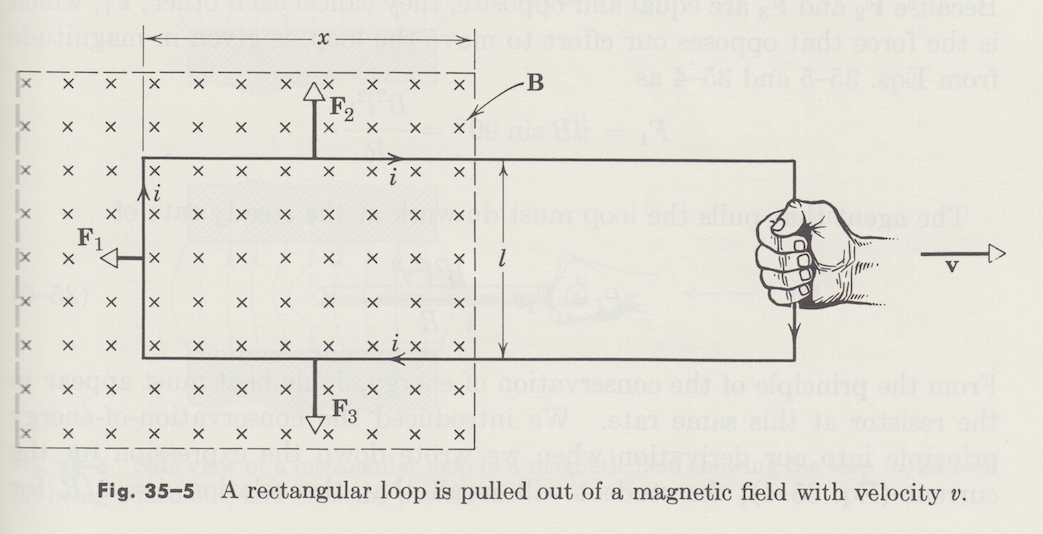
\includegraphics [scale=0.4] {induction.png} \end{center}
A uniform magnetic field is somehow produced that has a boundary.  The crosses show that the field points into the page.  A loop of wire is pulled through the edge of the field, and the movement causes a current to flow in the loop.

If a current is flowing there must be an EMF ($\mathcal{E}$).  The force is
\[ \mathcal{E} = \oint (\mathbf{v} \times \mathbf{B}) \cdot d\mathbf{l} \]
As the drawing indicates, the force points perpendicular to the wire.  This means that the forces on the top and bottom cancel.  It is the unbalanced force on the left-hand side of the loop that makes the current flow.  Work is applied to move the loop, this energy input appears as heat in the wire.

One way to figure out which way the current will flow is to remember that the induced current will itself cause a magnetic field.  This field will be such as to \emph{counteract the existing field} $\mathbf{B}$.  In this loop, the current will flow clockwise, as indicated by the little arrows.  The field due to the loop points out of the page.
\[ \mathcal{E} = \oint \mathbf{E} + (\mathbf{v} \times \mathbf{B}) \cdot d\mathbf{l} = - \frac{d\Phi}{dt} \]
The minus sign is due to Lenz.

Another way to get current to flow would be to vary the magnetic field.  The flux resolves into two components:

\[ - \frac{d\Phi}{dt}=  -\iint_S \frac{\partial \mathbf{B}}{\partial t} \cdot d\mathbf{A} + \oint (\mathbf{v} \times \mathbf{B}) \cdot d\mathbf{l} \]

By subtraction
\[ \oint \mathbf{E} \cdot d\mathbf{l} = -\iint_S \frac{\partial \mathbf{B}}{\partial t} \cdot d\mathbf{A} \]
through Stokes' theorem we obtain
\[ \iint_S \nabla \times \mathbf{E} \cdot d\mathbf{A} = -\iint_S \frac{\partial \mathbf{B}}{\partial t} \cdot d\mathbf{A} \] 
so the same trick as before gives
\[ \nabla \times \mathbf{E} = - \frac{\partial \mathbf{B}}{\partial t}  \]

\subsection*{Maxwell's Equations}
\[ \nabla \cdot \mathbf{E} = \frac{1}{\epsilon_0} \rho \]
\[ \nabla \cdot \mathbf{B} = 0 \]
\[ \nabla \times \mathbf{B} = \mu_0 (\mathbf{j} + \epsilon_0 \frac{\partial \mathbf{E}}{\partial t} )  \]
\[ \nabla \times \mathbf{E} = - \frac{\partial \mathbf{B}}{\partial t}  \]

In free space there is no charge and no current so we have just
\[ \nabla \cdot \mathbf{E} = 0 \]
\[ \nabla \cdot \mathbf{B} = 0 \]
\[ \nabla \times \mathbf{B} = \mu_0 \epsilon_0 \ \frac{\partial \mathbf{E}}{\partial t}  \]
\[ \nabla \times \mathbf{E} = - \frac{\partial \mathbf{B}}{\partial t}  \]

\subsection*{wave equation}
Now, suppose there is an electric field and a magnetic field at right angles to each other.  
\begin{center} 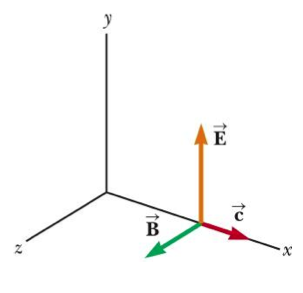
\includegraphics [scale=0.6] {EB_lightwave.png} \end{center}
The electric field $\mathbf{E}$ is all in the $y$-direction, while the magnetic field $\mathbf{B}$ is all in the $z$-direction.  Both fields are functions of $x$ and $t$, and we are only concerned with what happens close to the $x$-axis.  We compute the curl of both fields
\[ \nabla \times \mathbf{E} = 
\begin{vmatrix}  
\hat{\mathbf{i}} & \hat{\mathbf{j}} & \hat{\mathbf{k}}  \\  
\frac{\partial}{\partial x}  & \frac{\partial}{\partial y} & \frac{\partial}{\partial z} \\
0 & \mathbf{E}(x,t) & 0
\end{vmatrix}
= | \frac{\partial \mathbf{E}}{\partial x} |  \ \hat{\mathbf{k}}  \]
Thus by one of our fundamental equations
\[ \nabla \times \mathbf{E} = \frac{\partial \mathbf{E}}{\partial x} =  - \frac{\partial \mathbf{B}}{\partial t}  \]
Similarly
\[ \nabla \times \mathbf{B} = 
\begin{vmatrix}  
\hat{\mathbf{i}} & \hat{\mathbf{j}} & \hat{\mathbf{k}}  \\  
\frac{\partial}{\partial x}  & \frac{\partial}{\partial y} & \frac{\partial}{\partial z} \\
0 & 0 & \mathbf{B}(x,t)
\end{vmatrix}
= - | \frac{\partial \mathbf{B}}{\partial x} |  \ \hat{\mathbf{k}}  \]
Thus, by another of our fundamental equations
\[ \frac{\partial \mathbf{E}}{\partial t} = - \frac{1}{\mu_0 \epsilon_0} \ \nabla \times \mathbf{B} =  \frac{1}{\mu_0 \epsilon_0} \ \frac{\partial \mathbf{B}}{\partial x}  \]
Take the $x$-derivative of the first result
\[ \frac{\partial \mathbf{E}}{\partial x} =  - \frac{\partial \mathbf{B}}{\partial t}  \]
\[ \frac{\partial^2 \mathbf{E}}{\partial x^2} = \frac{\partial}{\partial x} \ (- \frac{\partial \mathbf{B}}{\partial t}) = \frac{\partial}{\partial t} \ (- \frac{\partial \mathbf{B}}{\partial x})  \]
\[ = - \frac{\partial}{\partial t} \ (\mu_0 \epsilon_0 \frac{\partial \mathbf{E}}{\partial t})  \]
\[ \frac{\partial^2 \mathbf{E}}{\partial x^2} = \mu_0 \epsilon_0 \ \frac{\partial^2 \mathbf{E}}{\partial t^2} \]
But we know this equation.  It is the wave equation.
\[ \frac{\partial^2 \mathbf{E}}{\partial x^2} =  \frac{1}{ c^2} \ \frac{\partial^2 \mathbf{E}}{\partial t^2} \]
\[ c^2 = \frac{1}{ \mu_0 \epsilon_0} \]

\subsection*{calculation}

\[ \mu_0 = 4 \pi \times 10^{-7} \]
\[ \epsilon_0 = 8.8542 \times 10^{-12} \]
\[ \frac{1}{ \mu_0 \epsilon_0} = \frac{1}{111.265 \times 10^{-19}}  \]
since $1/111.265 = 0.00898$
\[ c^2 = 8.99 \times 10^{16} \]
\[ c = 2.99 \times 10^8 \]

What about the units?

$\epsilon_0$ is in 
\[ \frac{\text{Farads }}{m} =  \frac{s^4 \cdot A^2}{m^3 \cdot \text{ kg}} \]

$\mu_0$ is in
\[ \frac{N}{A^{-2}} =  \frac{\text {kg } \cdot m}{s^{2} \cdot A^{2}} \]

The product is thus $s^2 / m^{2}$.  Invert and take the square root and we have meters per second, a velocity.  

The speed of light in a vacuum was known to be $2.99 \times 10^8 m/s$



\end{document}  